\documentclass{article}
\usepackage{note_preamble}

\usepackage{titling}
\setlength{\droptitle}{-2cm}


\lstset{style=python-style1}

\begin{document}
\title{Machine Learning Notes}
\author{Zach Virgilio}
\maketitle 

\section*{Makemore notes}
\subsection*{Diagnostic Tools and Visualization}
    \begin{enumerate}
        \item Activation saturation of non-linear layers, i.e. $\tanh$ or ReLu etc.  For $\tanh$ layers, want to make sure the distribution is fairly even, and not tailed towards $\pm 1$ like in:

        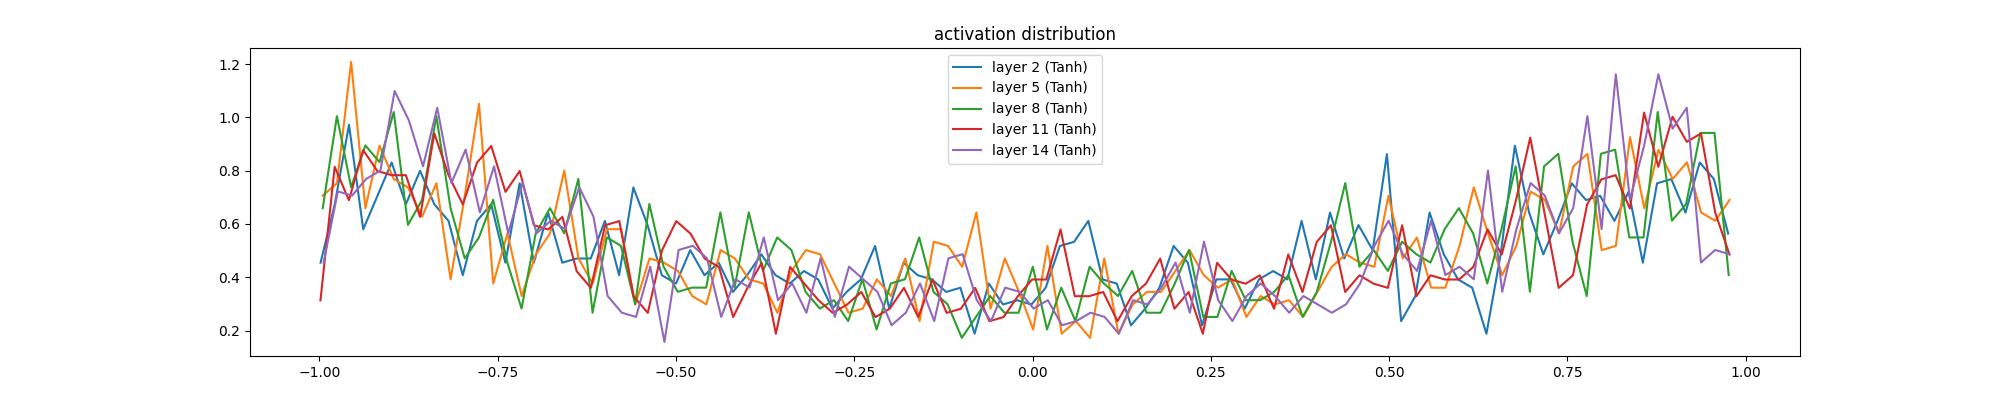
\includegraphics[width=0.9\textwidth]{images/tanh-activation}        

        Produced with \ref{code:activation-graph}.  
        This is important, because neurons with activations of $\pm 1$ will have gradients of $0$, as $\frac{d}{dx}\tanh x = 1 - (\tanh x)^2$, leading to dead neurons which don't learn. 
        The same phenomena occurs for sigmoid non-linearity.
        These are forward pass statistics

        \item Gradients of the non-linear layers.  For $\tanh$ they can look like:

        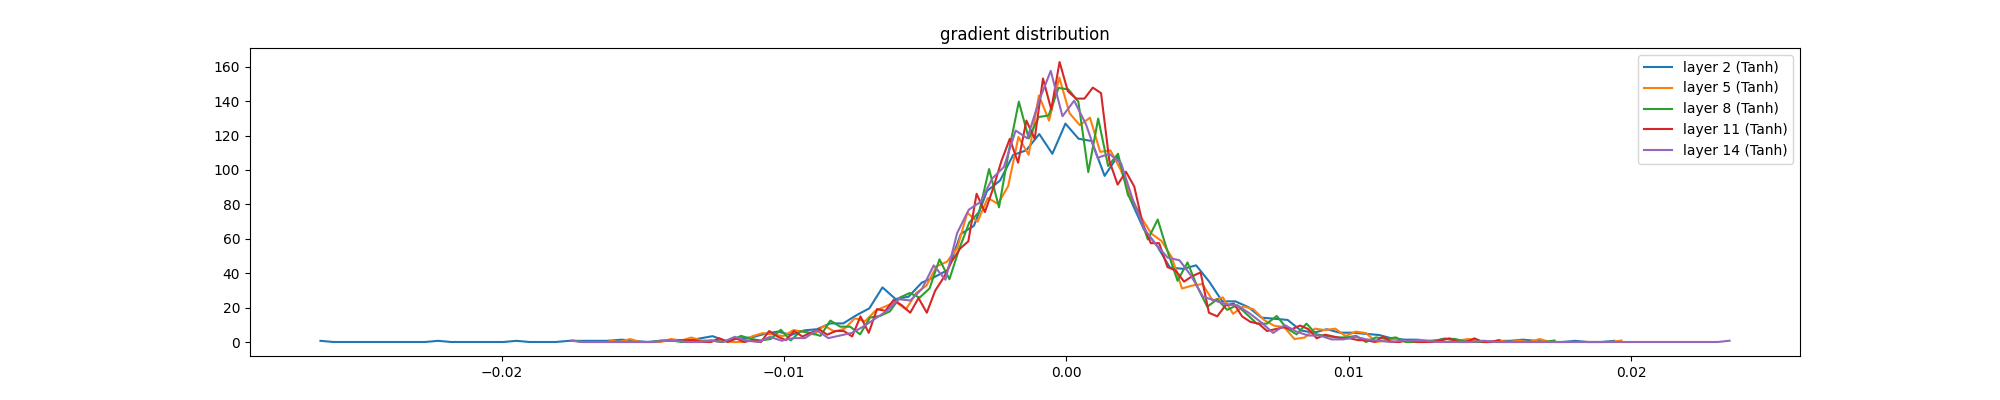
\includegraphics[width=0.9\textwidth]{images/dsitribution of gradients.png}

        Produced with \ref{code:grad-graph}.  These are backward pass statistics since they involve the gradient

        \item The ratio between the gradient and the parameter.  
        Should be similar for each layer after the first and before the last.  
        Restricting to 2-dim parameters, i.e. weights of the linear layers, not biases or $\gamma$ and $\beta$ in batch norm.

        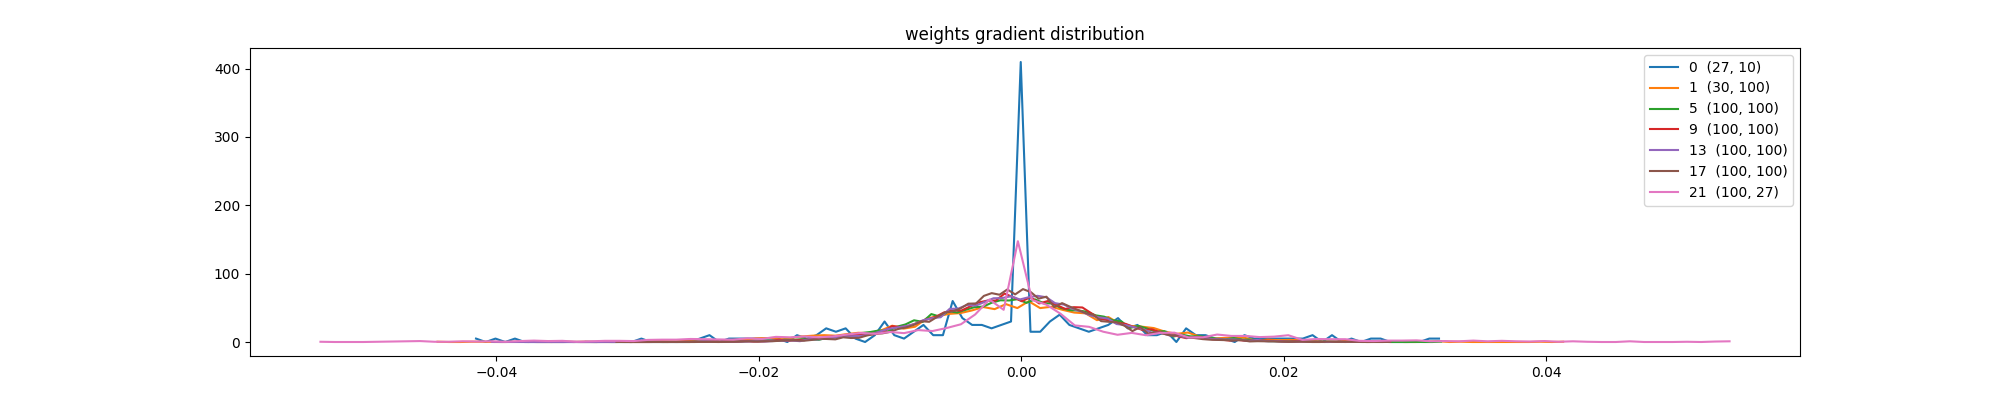
\includegraphics[width=0.9\textwidth]{images/grad-ratio.png}

        Produced with \ref{code:grad-scale-graph}.

        \item The size of the updates relative to the parameters.  
        As an estimate, want the $\log_{10}$ to be around $10^{-3}$. 
        This can be more informative than the gradient to data ratio, since what matters in learning is the size of the update.

        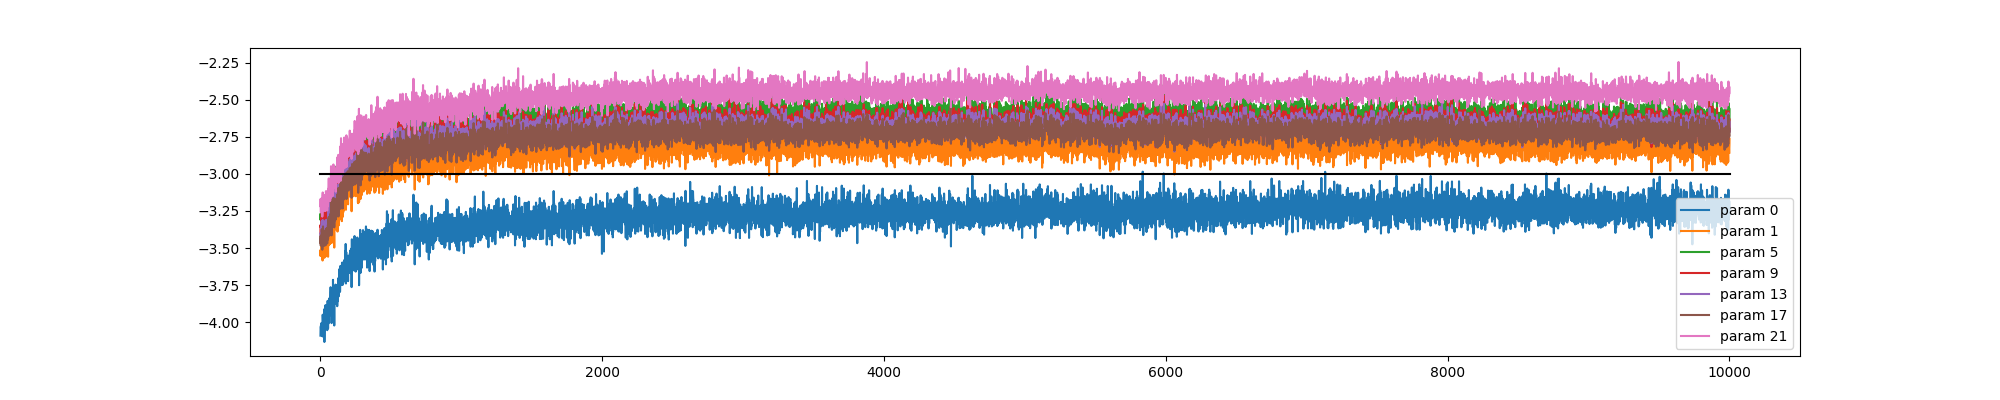
\includegraphics[width=0.9\textwidth]{images/update-ratio.png}

        Produced with \ref{code:update-graph}.
    \end{enumerate}

\begin{redbox}{Question}
    Why do we look at the ratio of grad standard deviations to parameter standard deviation (similarly for updates), instead of absolute values.
\end{redbox}

\subsection*{Batch Normalization}
Batch normalization is a technique used to stabilize training.  
It computes the mean and sd of the batch and uses that to normalize the batch to a standard normal distribution.  
This helps ensure neuron activation is more stable.
For example, if the non-linear layer is $\tanh$, it will take values of $\pm 1$ for inputs that are too far away from 0.  Oversaturation could keep some neurons always on or off.
It also means that adding a bias in a linear layer that comes before a batch normalization step is redundant as that bias is added to the norm and immediately subtracted, rendering it useless.


\subsection*{Backpropogation}
Be aware when a column is replicated before an elementwise operation is performed, you need to sum the gradients along the duplicated rows.
If a value $x$ feeds into to different paths, need to sum those gradients together.
Keep track to make sure torch broadcasting is properly backpropagated, this can be done by checking shape.

\subsection*{Containers}
Containers from PyTorch are ways of organizing layers into lists or dicts.  

\subsection*{Expiremental Harness}
When training takes longer and longer, need a way to test hyper-parameters such as learning rates and tune those without running the full training over and over.

\subsection*{Self attention trick}
\begin{lstlisting}[language=Python]    
import pytorch

torch.manual_seed(1337)
B, T, C = 4, 8, 2 # batch, time (block_size), channels (how many outputs)
x = torch.randn(B, T, C)
x.shape
\end{lstlisting}
want the 8 tokens in a block to 'talk' with each other.  
The fifth token in a block doesn't need info about sixth, seventh, eighth.  
Information only flows forwards in time.  We want the average of all the vectors corresponding to the previous tokens.  This is called \emph{bag of words} (bow).
\begin{lstlisting}[language=Python]
    xbow = torch.zeros((B, T, C))
    for b in range(B):
        for t in range(T):
            xprev = x[b,:t+1] # size (t, C)
            xbow[b,t] = torch.mean(xprev, 0)
\end{lstlisting}
But this is very inefficient.  
We can speed it up with matrix multiplication.

Recall:
\[
    \begin{bmatrix}
        1 & 1 & 1
    \end{bmatrix}\cdot 
    \begin{bmatrix}
        a & b & c
    \end{bmatrix} = a + b + c
\]
We can use a lower triangular matrix:
\[
    \begin{bmatrix}
        1 & 0 & 0 \\[1mm] \frac{1}{2} & \frac{1}{2} & 0 \\[1mm] \frac{1}{3} & \frac{1}{3} & \frac{1}{3}
    \end{bmatrix}\cdot 
    \begin{bmatrix}
        a & d \\ b & e \\ c & f
    \end{bmatrix} = \begin{bmatrix}
        \begin{bmatrix}
            1 & 0 & 0
        \end{bmatrix}\cdot 
        \begin{bmatrix}
            a & b & c
        \end{bmatrix} & 
        \begin{bmatrix}
            1 & 0 & 0
        \end{bmatrix}\cdot 
        \begin{bmatrix}
            d & e & f
        \end{bmatrix} \\[1mm]  
        \begin{bmatrix}
            \frac{1}{2} & \frac{1}{2} & 0
        \end{bmatrix}\cdot 
        \begin{bmatrix}
            a & b & c
        \end{bmatrix} & 
        \begin{bmatrix}
            \frac{1}{2} & \frac{1}{2} & 0
        \end{bmatrix}\cdot 
        \begin{bmatrix}
            d & e & f
        \end{bmatrix} \\[1mm] 
        \begin{bmatrix}
            \frac{1}{3} & \frac{1}{3} & \frac{1}{3}
        \end{bmatrix}\cdot 
        \begin{bmatrix}
            a & b & c
        \end{bmatrix} & 
        \begin{bmatrix}
            \frac{1}{3} & \frac{1}{3} & \frac{1}{3}
        \end{bmatrix}\cdot 
        \begin{bmatrix}
            d & e & f
        \end{bmatrix}  
    \end{bmatrix} = 
    \begin{bmatrix}
        a & d \\[1mm] \frac{a+b}{2} & \frac{d+e}{2} \\[1mm] \frac{a+b+c}{3} & \frac{d+e+f}{3}
    \end{bmatrix}
\]
We can instantly compute the averages.
This lets us vectorize the previous process:
\begin{lstlisting}[language=Python]
    wei = torch.tril(torch.ones(T, T)) # tril = triangular, lower
    wei = wei / wei.sum(1, keepdim=True) # divide by each rows total
    xbow2 = wei @ x 
\end{lstlisting}
The dimensions don't line up, we have: $(T, T)\cdot (B, T, C)$.  
So torch will replicate the $(T, T)$ $B$ many times giving dimensions: $(B, T, T) \cdot (B, T, C)$ and then multiply each batch element in parallel, so we have a $(T, T)\cdot (T, C) = (T, C)$ computation for each element in the batch $B$.

There is a third way to do this, using \emph{softmax}.
\begin{lstlisting}[language=Python]
    tril = torch.tril(torch.ones(T, T))
    wei = torch.zeros(T, T)
    wei = wei.masked_fill(tril == 0, float('-inf')) #all elements that are zero in tril (lower triangular) become -infinity
    wei = F.softmax(wei, dim=-1) # e to each value, then normalize the rows to sum to 1
    xbow3 = wei @ x
\end{lstlisting}
Can generalize this idea to more general weighted averages based on how important some past tokens are to the current token.  

Here is the implementation for a single self attention head.
Every single token will emit two vectors: a query vector and a key vector.
The query vector is 'what am I looking for', the key vectors is 'what do I contain'.
The query vector of a token dot products with the key vector of all previous tokens in the block and this should be the information stored in \emph{wei}, the weights.  If the key and query are aligned (in space, which should be learned), their dot product will be high, ensuring that the previous token with that key has more influence on the current vector querying the context.

We also produce a \emph{value} parameter.  We don't aggregate $x$, instead we aggregate value applied to $x$.

Attention is a communcation mechanism between nodes in a direct graph.  A given node aggregates information with a weight sum from all the nodes that point towards it.
There is no notion of space (such as in convolution).  Attention simply acts over a set of vectors, hence the need to positionally encode tokens.
This is why there is a positional encoding added to the token embeddedings.
You don't need to have the lower triangular masking in more general settings, such as in an encoder block in sentiment analysis.

Self-attention because keys, querys and values all come from the same $x$. In general, you could have a case where querys come from $x$, but keys and values come from an external source of context, where would like to pull that into our nodes.

Scaled attention divides $QK^T$ by $\sqrt{\textit{head size}}$. This preverves the variance of \emph{wei} at 1. 
This is important, especially at initialization, to ensure that \emph{wei} has diffuse values.  
When being fed into \emph{softmax}, any values that are too positive or negative will cause \emph{wei} to converge to one-hot vectors.
\begin{lstlisting}[language=Python]
import torch
import torch.nn as nn
from torch.nn import functional as F

torch.manual_seed(1337)

B, T, C = 4, 8, 32 # batch, time (block_size), channels (how many outputs)
x = torch.randn(B, T, C)

# single head self-attention
head_size = 16 # this is a hyper parameter
key = nn.Linear(C, head_size, bias=False) #linear layer with no bias is a matrix multiply with fixed weights
query = nn.Linear(C, head_size, bias=False)
value = nn.Linear(C, head_size, bias=False)
k = key(x)      # (B, T, 16)
q = query(x)    # (B, T, 16)

# this is the step where the communication occurs
wei = q @ k.transpose(-2, -1) # transpose last two dimensions, not the first (B, T, 16) @ (B, 16, T) --> (B, T, T)
wei = wei * head_size**-0.5   # scaled attention

tril = torch.tril(torch.ones(T, T))
wei = wei.masked_fill(tril == 0, float('-inf')) #all elements that are zero in tril (lower triangular) become -infinity
wei = F.softmax(wei, dim=-1) # e to each value, then normalize the rows to sum to 1

v = value(x)    # (B, T, 16)
out = wei @ v   # (B, T, T) @ (B, T, 16) --> (B, T, 16)
\end{lstlisting}

\subsection*{Residual Connections}
When training very large/deep neural networks, optimization begins to degrade with size.
This is not explained by overfitting along, as even training errors grows.
A way to counter this is with residual connections, where identity blocks are added in.
The blocks take the inputs, unaltered, and add them to outputs at later stages in the training.  
This ensures that performance does not become worse.
It also places little strain on optimization as the gradient of addition is simple.
You can fork off the residual pathway at will, and project back in by addition.
The blocks that fork off are intialized to have very small gradients, so early on in training there is a quick gradient path back from the outputs to the inputs.
Only later in training do these blocks come on line.
You want a clean residual stream, no normalizations inside {\color{mred} why? This is a quote from Karpathy}.

Dropout layers prevent overfitting.  Every forward/backward pass, randomly turns off some neurons, ends up training an ensamble of networks that all end up working together.

\section*{Makemore Code Snippets}
\begin{lstlisting}[language=Python, caption={Activation graph with matplotlib}, label={code:activation-graph}]    
# visualize histograms of layer activation
plt.figure(figsize=(20, 4))
legends = []

for i, layer in enumerate(layers[:-1]): #exclude output layer
    if isinstance(layer, Tanh):
        t = layer.out 
        print('layer %d (%10s): mean %+.2f, std %.2f, saturated: %.2f%%' % (i, 
                layer.__class__.__name__, 
                t.mean(), t.std(), 
                (t.abs()>0.97).float().mean()*100))
        hy, hx = torch.histogram(t, density=True)
        plt.plot(hx[:-1].detach(), hy.detach())
        legends.append(f'layer {i} ({layer.__class__.__name__})')
plt.legend(legends)
plt.title('activation distribution')
# plt.show()
\end{lstlisting}

\begin{lstlisting}[language=Python, caption={Gradients of $\tanh$ layers with matplotlib}, label={code:grad-graph}]
    # histogram of gradients
plt.figure(figsize=(20, 4))
legends = []
for i, layer in enumerate(layers[:-1]): #exclude output layer
    if isinstance(layer, Tanh):
        t = layer.out.grad
        print('layer %d (%10s): mean %+.2f, std %e' % (i, 
                layer.__class__.__name__, 
                t.mean(), t.std()))
        hy, hx = torch.histogram(t, density=True)
        plt.plot(hx[:-1].detach(), hy.detach())
        legends.append(f'layer {i} ({layer.__class__.__name__})')
plt.legend(legends)
plt.title('gradient distribution')
\end{lstlisting}

\begin{lstlisting}[language=Python, caption={Scale between gradients and values of parameters}, label={code:grad-scale-graph}]
# parameter values visualization
# scale of gradient compared to actual values
plt.figure(figsize=(20, 4))
legends = []
for i, p in enumerate(parameters): #exclude output layer
    t = p.grad 
    if p.ndim == 2:
        print('weight %10s | mean %+f | std %e | grad:data ration %e' % (tuple(p.shape), 
                t.mean(), t.std(), t.std() / p.std() ))
        hy, hx = torch.histogram(t, density=True)
        plt.plot(hx[:-1].detach(), hy.detach())
        legends.append(f'{i}  {tuple(p.shape)}')
plt.legend(legends)
plt.title('weights gradient distribution')
\end{lstlisting}

\begin{lstlisting}[language=Python, caption={Size of update scaled by size of the parameter}, label={code:update-graph}]
#before training code
ud=[]
##### TRAINING #####
# in training loop
# lr is learning rate
# this tracks the log base 10
with torch.no_grad():
        ud.append([(lr*p.grad.std() / p.data.std()).log10().item() for p in parameters])
####################
# at each update, keep track of log of update size compated to data size
# these should be low or else we are over updating
# last layer can be large since that layer was ariticially compressed
plt.figure(figsize=(20,4))
legends = []
for i,p in enumerate(parameters):
    if p.ndim == 2:
        plt.plot([ud[j][i] for j in range(len(ud))])
        legends.append('param %d' % i)
plt.plot([0, len(ud)], [-3, -3], 'k') # ratios should be 1e-3
plt.legend(legends)
plt.show()
\end{lstlisting}
\end{document}